\documentclass[twoside,openright,titlepage,fleqn,
	headinclude,11pt,a4paper,BCOR5mm,footinclude
	]{scrbook}
%--------------------------------------------------------------
        \newcommand{\myTitle}{Formal methods for systems verification\xspace}
% use the right myDegree option
\newcommand{\myDegree}{Corso di Laurea Magistrale in Informatica\xspace}
%\newcommand{\myDegree}{
	%Corso di Laurea Specialistica in Scienze e Tecnologie 
	%dell'Informazione\xspace}
\newcommand{\myName}{Massimo Nocentini\xspace}
\newcommand{\myProf}{Michele Loreti\xspace}
\newcommand{\myOtherProf}{Mieke Massink\xspace}
\newcommand{\mySupervisor}{Nome Cognome\xspace}
\newcommand{\myFaculty}{
	Facolt\`a di Scienze Matematiche, Fisiche e Naturali\xspace}
\newcommand{\myDepartment}{
	Dipartimento di Sistemi e Informatica\xspace}
\newcommand{\myUni}{\protect{
	Universit\`a degli Studi di Firenze}\xspace}
\newcommand{\myLocation}{Firenze\xspace}
\newcommand{\myTime}{Anno Accademico 2012-2013\xspace}
\newcommand{\myVersion}{Version 0.1\xspace}

%--------------------------------------------------------------
\usepackage[latin1]{inputenc} 
\usepackage[T1]{fontenc} 
\usepackage[square,numbers]{natbib} 
\usepackage[fleqn]{amsmath}  
\usepackage[english]{babel}
\usepackage{ae,aecompl}
\usepackage[pdftex]{graphicx}
\usepackage{latexsym}
\usepackage{amsmath, amsthm, amssymb}
\usepackage{rotating}
\usepackage{boxedminipage}
\usepackage{multicol}

%--------------------------------------------------------------
\usepackage{dia-classicthesis-ldpkg} 
%--------------------------------------------------------------
% Options for classicthesis.sty:
% tocaligned eulerchapternumbers drafting linedheaders 
% listsseparated subfig nochapters beramono eulermath parts 
% minionpro pdfspacing
\usepackage[eulerchapternumbers,subfig,beramono,eulermath,
	parts]{classicthesis}
%--------------------------------------------------------------
\newlength{\abcd} % for ab..z string length calculation
% how all the floats will be aligned
\newcommand{\myfloatalign}{\centering} 
\setlength{\extrarowheight}{3pt} % increase table row height
\captionsetup{format=hang,font=small}
%--------------------------------------------------------------
% Layout setting
%--------------------------------------------------------------
\usepackage{geometry}
\geometry{
	a4paper,
	ignoremp,
	bindingoffset = 1cm, 
	textwidth     = 13.5cm,
	textheight    = 21.5cm,
	lmargin       = 3.5cm, % left margin
	tmargin       = 4cm    % top margin 
}
%--------------------------------------------------------------

\usepackage{hyperref}
\usepackage{listings}
\usepackage{pdfpages}
% My Theorem
\newtheorem{oss}{Observation}[section]
\newtheorem{exercise}{Exercise}[section]
\newtheorem{thm}{Theorem}[section]
\newtheorem{cor}[thm]{Corollary}

\newtheorem{lem}[thm]{Lemma}

\newcommand{\vect}[1]{\boldsymbol{#1}}

% questo comando e' relativo alle correzioni che puo
% apportare il prof se lo desidera.
\newcommand{\prof}[1]{\boldsymbol{#1}}

% instead of boldsymbol I can use the arrow above the letter with
%\newcommand{\vect}[1]{\vec{#1}}

% page settings
% \pagestyle{headings}
%--------------------------------------------------------------
\begin{document}
\frenchspacing
\raggedbottom
\pagenumbering{roman}
\pagestyle{plain}
%--------------------------------------------------------------
% Frontmatter
%--------------------------------------------------------------
%--------------------------------------------------------------
% titlepage.tex (use thesis.tex as main file)
%--------------------------------------------------------------
\begin{titlepage}
	\begin{center}
   	\large
      \hfill
      \vfill
      \begingroup
			\spacedallcaps{\myUni} \\ 
			\myFaculty \\
			\myDegree \\ 
			\vspace{0.5cm}
         
\includegraphics[scale=.065]{logo/unifi}\\
         \vspace{0.5cm}    
         %% -------put here the type of document---ie: Tesi di Laurea
         Elaborato d'Esame
      \endgroup 
      \vfill 
      \begingroup
      	\color{Maroon}\spacedallcaps{\myTitle} \\ \bigskip
      \endgroup
      \spacedlowsmallcaps{\myName}
      \vfill  
      Professori: \itshape{\myProf}, \itshape{\myOtherProf}
      \vfill  
      \myTime
      \vfill                      
	\end{center}        
\end{titlepage}   
%--------------------------------------------------------------
% back titlepage
%--------------------------------------------------------------
   \newpage
	\thispagestyle{empty}
	\hfill
	\vfill
	\noindent\myName: 
	\textit{\myTitle,} 
	\myDegree, \textcopyright\ \myTime
%--------------------------------------------------------------
% back titlepage end
%--------------------------------------------------------------
\pagestyle{scrheadings}
%--------------------------------------------------------------
% Mainmatter
%--------------------------------------------------------------
\pagenumbering{arabic}

% settings for the lstlisting environment
\lstset{
	language = R
	, numbers = left 
	, basicstyle=\sffamily%\footnotesize
%	, frame=single
	, tabsize=2
	, captionpos=b
	, breaklines=true
	, showspaces=false
	, showstringspaces=false
}

\tableofcontents

\newpage

\section*{Goal}
This document collects my work on the course \emph{Formal methods for
  system verification}.

\subsection*{Some useful web location}
The source of the exercises is:\\
\href{http://www-i2.informatik.rwth-aachen.de/i2/mvps11/}{
  http://www-i2.informatik.rwth-aachen.de/i2/mvps11/}
\\\\
This document is hosted in the following \texttt{git} repository:
\\
\href{https://github.com/massimo-nocentini/metodi-formali-verifica-sistemi}{
  https://github.com/massimo-nocentini/metodi-formali-verifica-sistemi}


\newpage

\section*{Licences}

\subsection*{Text contents}
All the text content is distributed under:\\
\textbf{ This work is licensed under the Creative Commons Attribution,
  NonCommercial, ShareAlike 3.0 Unported License. To view a
  copy of this license, visit\\
  \href{http://creativecommons.org/licenses/by-nc-sa/3.0/}{http://creativecommons.org/licenses/by-nc-sa/3.0/}\\
  or send a letter to Creative Commons, 444 Castro Street, Suite 900,
  Mountain View, California, 94041, USA.}

\begin{center}
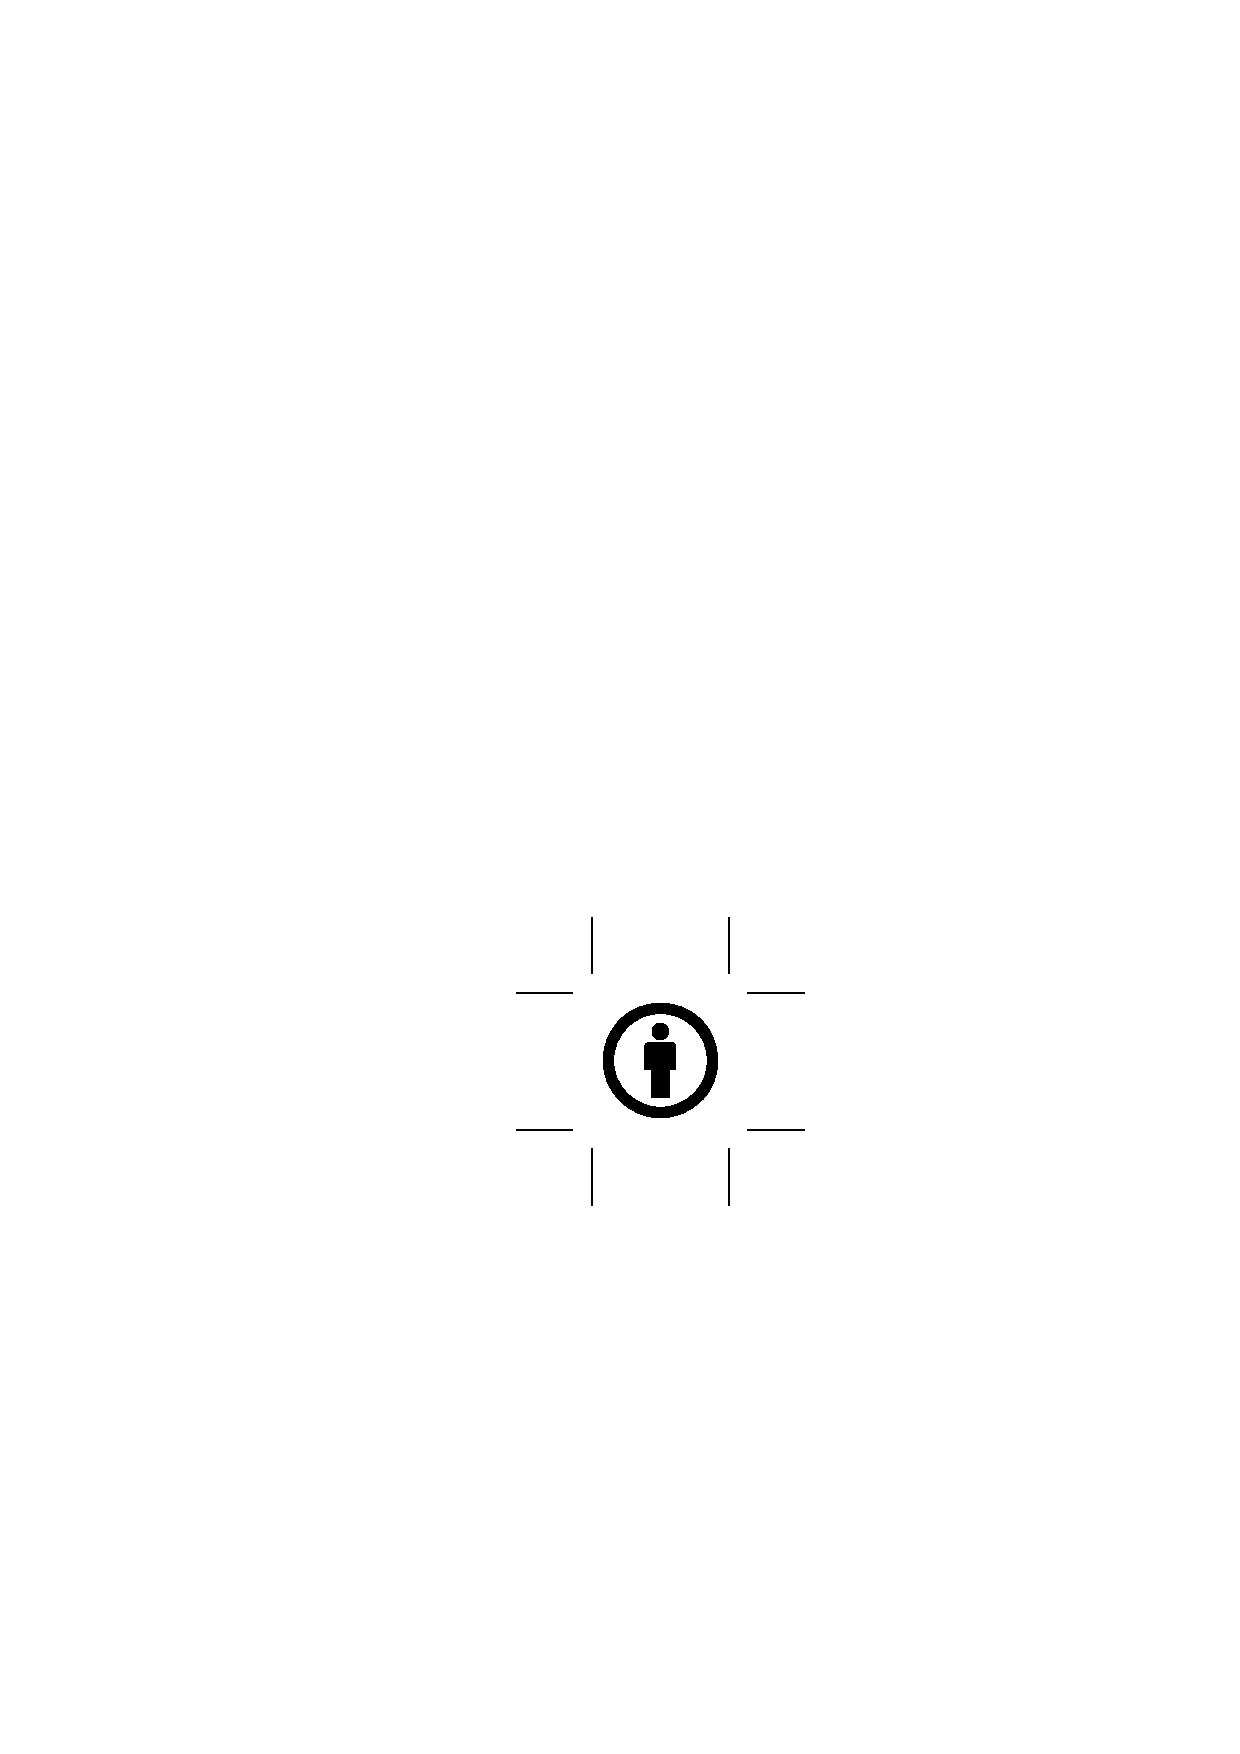
\includegraphics{cc-icons-eps/by}
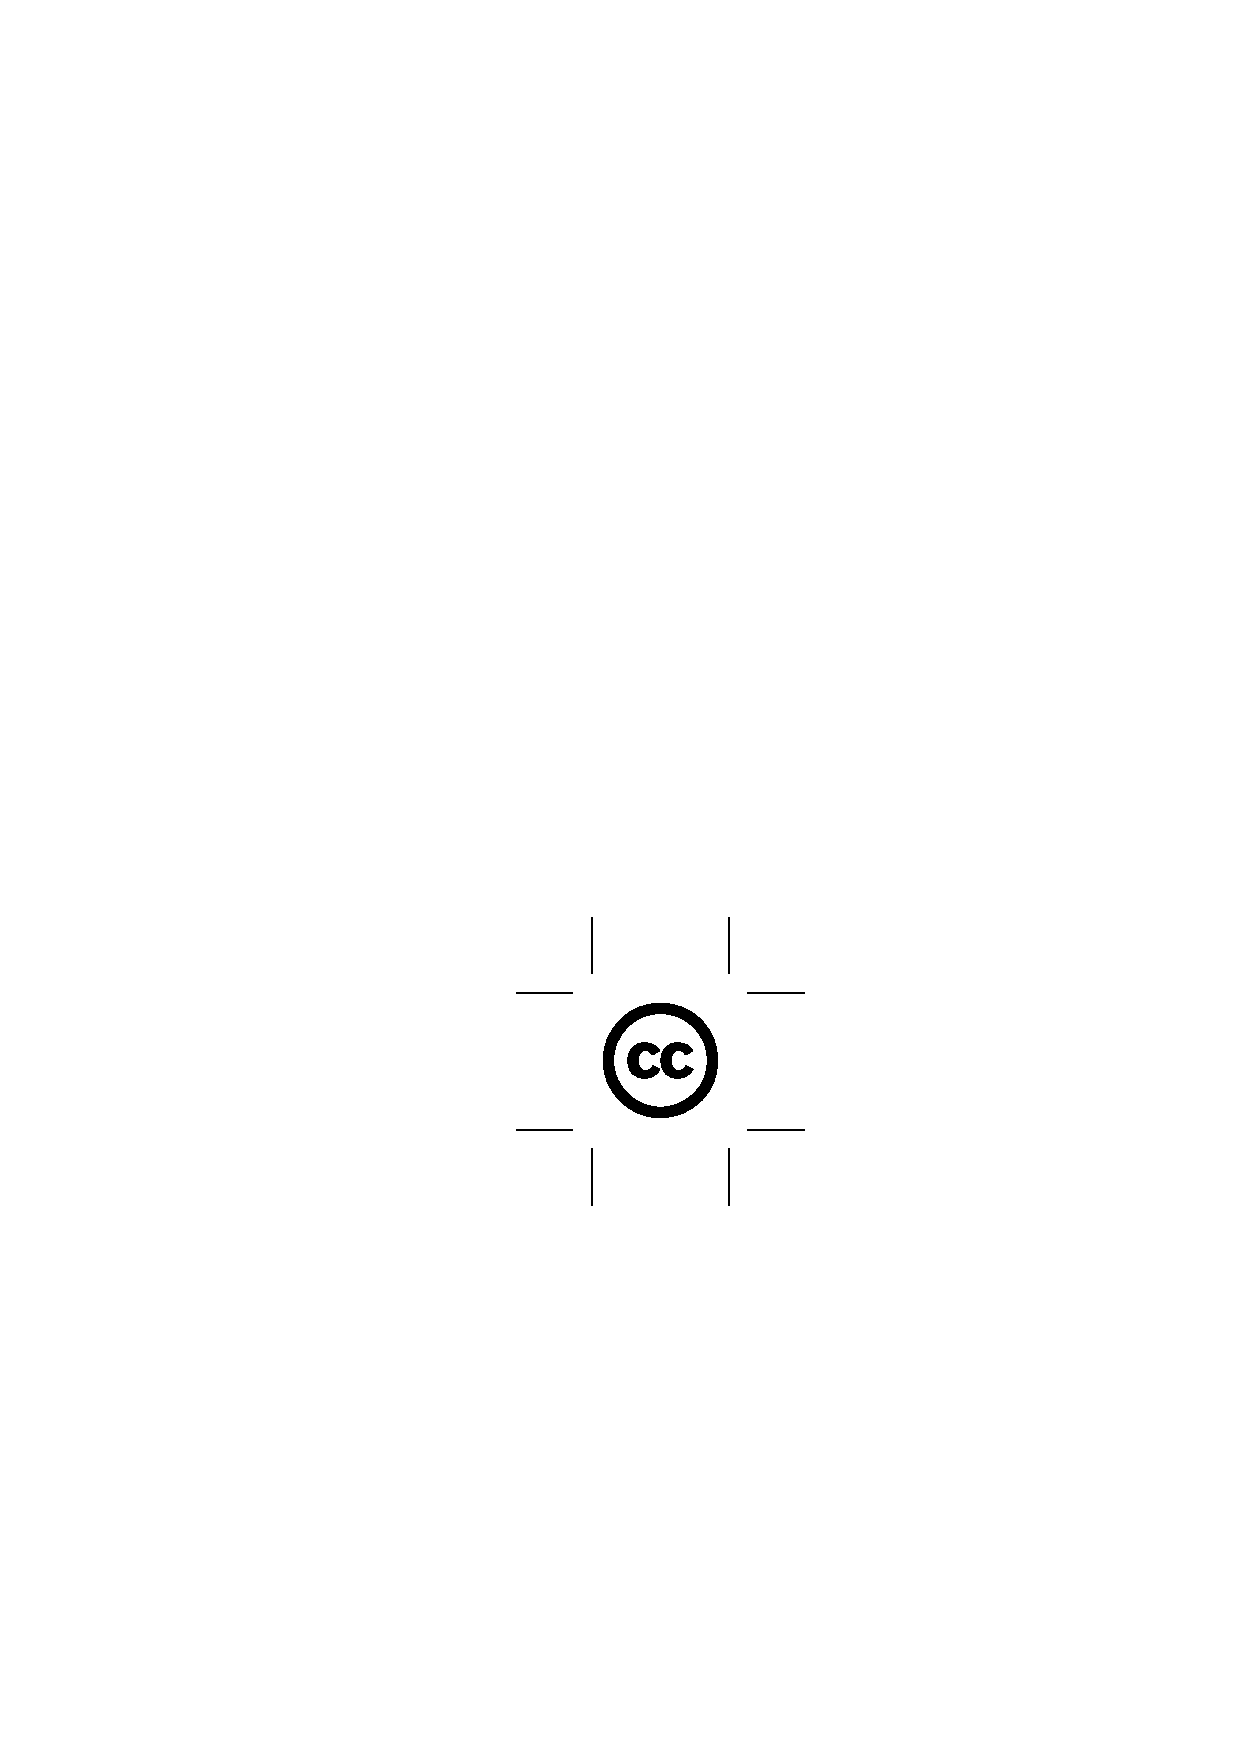
\includegraphics{cc-icons-eps/cc}
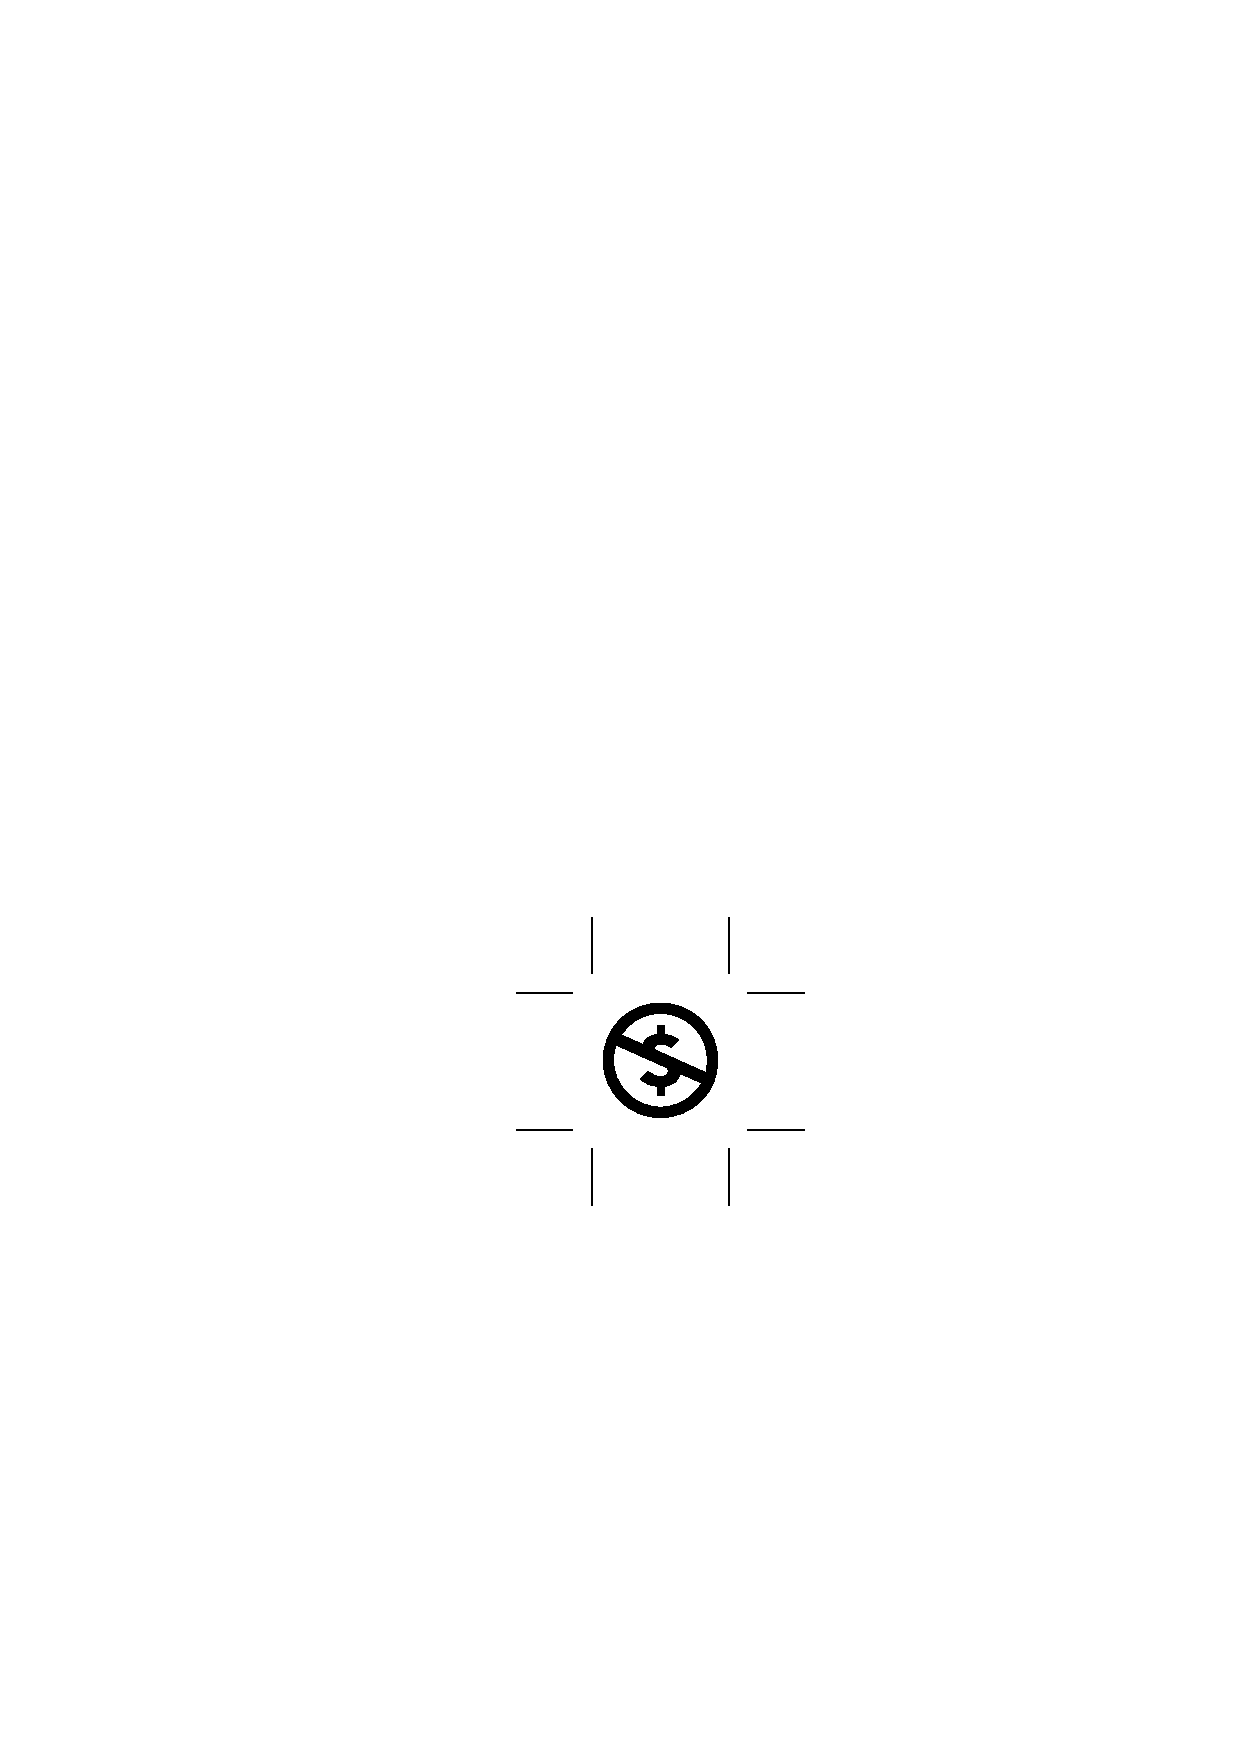
\includegraphics{cc-icons-eps/nc}
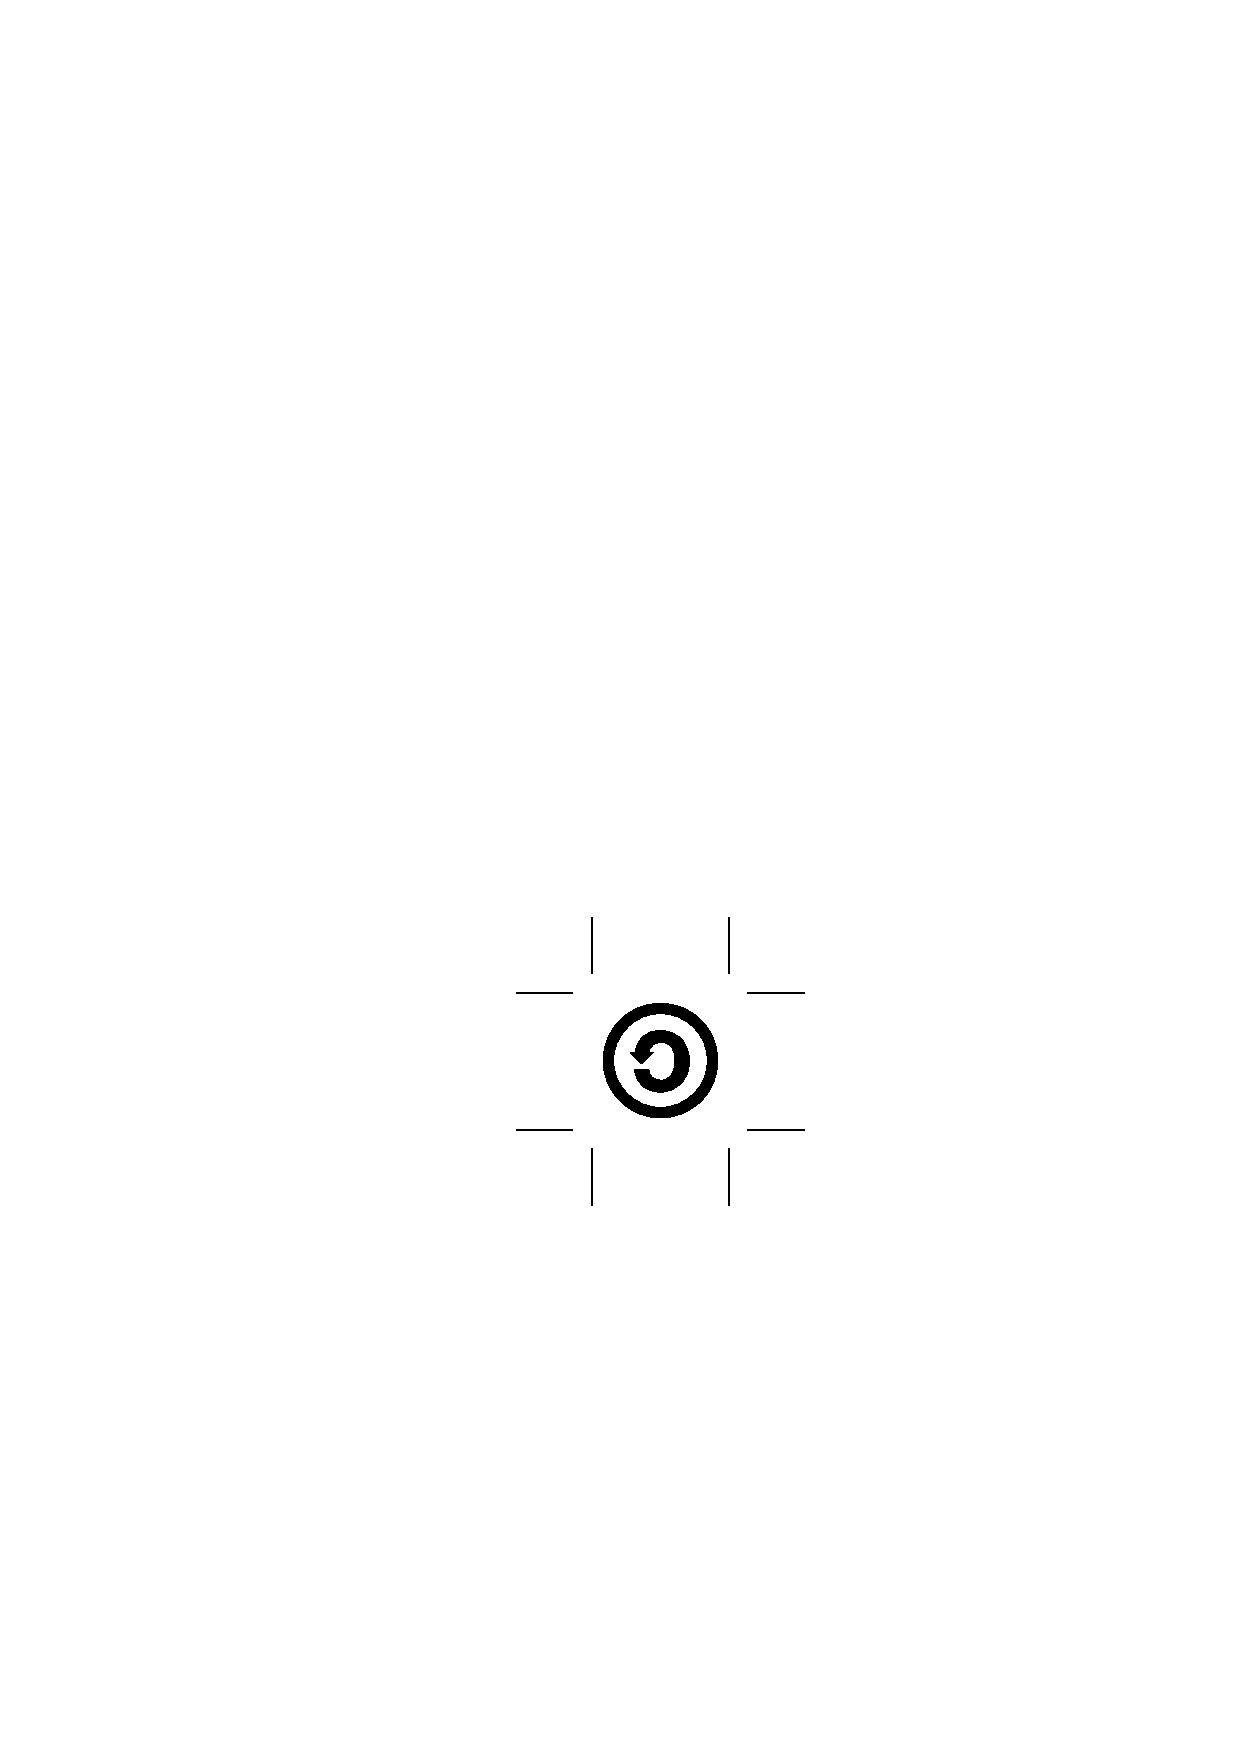
\includegraphics{cc-icons-eps/sa}
\end{center}

\subsection*{Sources}
All sources are distributed under, where the word ``Software'' is
referred to all of the sources that are present in this work: \\
\textbf{
  Copyright (c) 2011 Massimo Nocentini\\
  Permission is hereby granted, free of charge, to any person
  obtaining a copy of this software and associated documentation files
  (the "Software"), to deal in the Software without restriction,
  including without limitation the rights to use, copy, modify, merge,
  publish, distribute, sublicense, and/or sell copies of the Software,
  and to permit persons to whom the Software is furnished
  to do so, subject to the following conditions:\\
  The above copyright notice and this permission notice shall be
  included in all
  copies or substantial portions of the Software.\\
  THE SOFTWARE IS PROVIDED "AS IS", WITHOUT WARRANTY OF ANY KIND,
  EXPRESS OR IMPLIED, INCLUDING BUT NOT LIMITED TO THE WARRANTIES OF
  MERCHANTABILITY, FITNESS FOR A PARTICULAR PURPOSE AND
  NONINFRINGEMENT. IN NO EVENT SHALL THE AUTHORS OR COPYRIGHT HOLDERS
  BE LIABLE FOR ANY CLAIM, DAMAGES OR OTHER LIABILITY, WHETHER IN AN
  ACTION OF CONTRACT, TORT OR OTHERWISE, ARISING FROM, OUT OF OR IN
  CONNECTION WITH THE SOFTWARE OR THE USE OR OTHER DEALINGS IN THE
  SOFTWARE.  }


\chapter{Some exercises}

\section{Series 1}
\subsection{Exercise 1}
\subsubsection{Question a}
The set $\mathcal{F}$ is built according the following rules, $\forall
A \subseteq \Omega$, with $\Omega$ a countably infinite set:
\begin{enumerate}
\item $|A| < \infty \rightarrow A \in \mathcal{F}$
\item $A \in \mathcal{F} \rightarrow A^c \in \mathcal{F}$
\end{enumerate}
\begin{proof}
  We try to make some attempt to study the minimal composition of
  $\mathcal{F}$, induced by its definition.

  By rule 1, $\emptyset \in \mathcal{F}$ holds because $|\emptyset| <
  \infty$. By rule 2 follow $\Omega \in \mathcal{F}$, because
  $\emptyset \in \mathcal{F}$ and $\Omega = \emptyset^c$. So far we
  have $\mathcal{F} = \{\emptyset, \Omega \}$. Using rule 1 again,
  every finite set $A \subset \Omega$ belong to $\mathcal{F}$, hence
  $\mathcal{F} = \{\emptyset, \Omega \} \cup \{A \subset \Omega:
  |A|<\infty\}$. But the sets we added in the last step in
  $\mathcal{F}$ allow us to apply rule 2 on each of them, forcing to
  add the complement of each: $\mathcal{F} = \{\emptyset, \Omega \}
  \cup \{A \subset \Omega: |A|<\infty\} \cup \{A^c \subset \Omega:
  |A|<\infty\}$ (note that the set $A^c$ is infinite where $A$ is
  finite and $\Omega$ is coutably infinite).

  The definition of $\mathcal{F}$ doesn't allow to add any other sets,
  hence we stop here in its construction.

  To show that $\mathcal{F}$ is not trivial, we have to show that
  exists a set which is in $2^{\Omega}$ but not in $\mathcal{F}$. In
  order to find such set, we have to exclude any finite set because by
  definition and the argument described above, it belong to
  $\mathcal{F}$. Hence it must be an infinite set. But we cannot
  choose an infinite set which is the complement of a finite one,
  otherwise it is in $\mathcal{F}$ too. Hence the choice restrict to
  an infinite set $A$ such that both $A$ both $A^c$ (which is infinite
  too, otherwise $A \in \mathcal{F}$ by rule 1) are not in
  $\mathcal{F}$. The set that contains every pair of sets $A$ and
  $A^c$, both infinite, is $2^\Omega$ and this finish the proof.
\end{proof}
To make an example choose $\Omega = \mathbb{N}, A = \{2i:i \in
\mathbb{N}\}$.

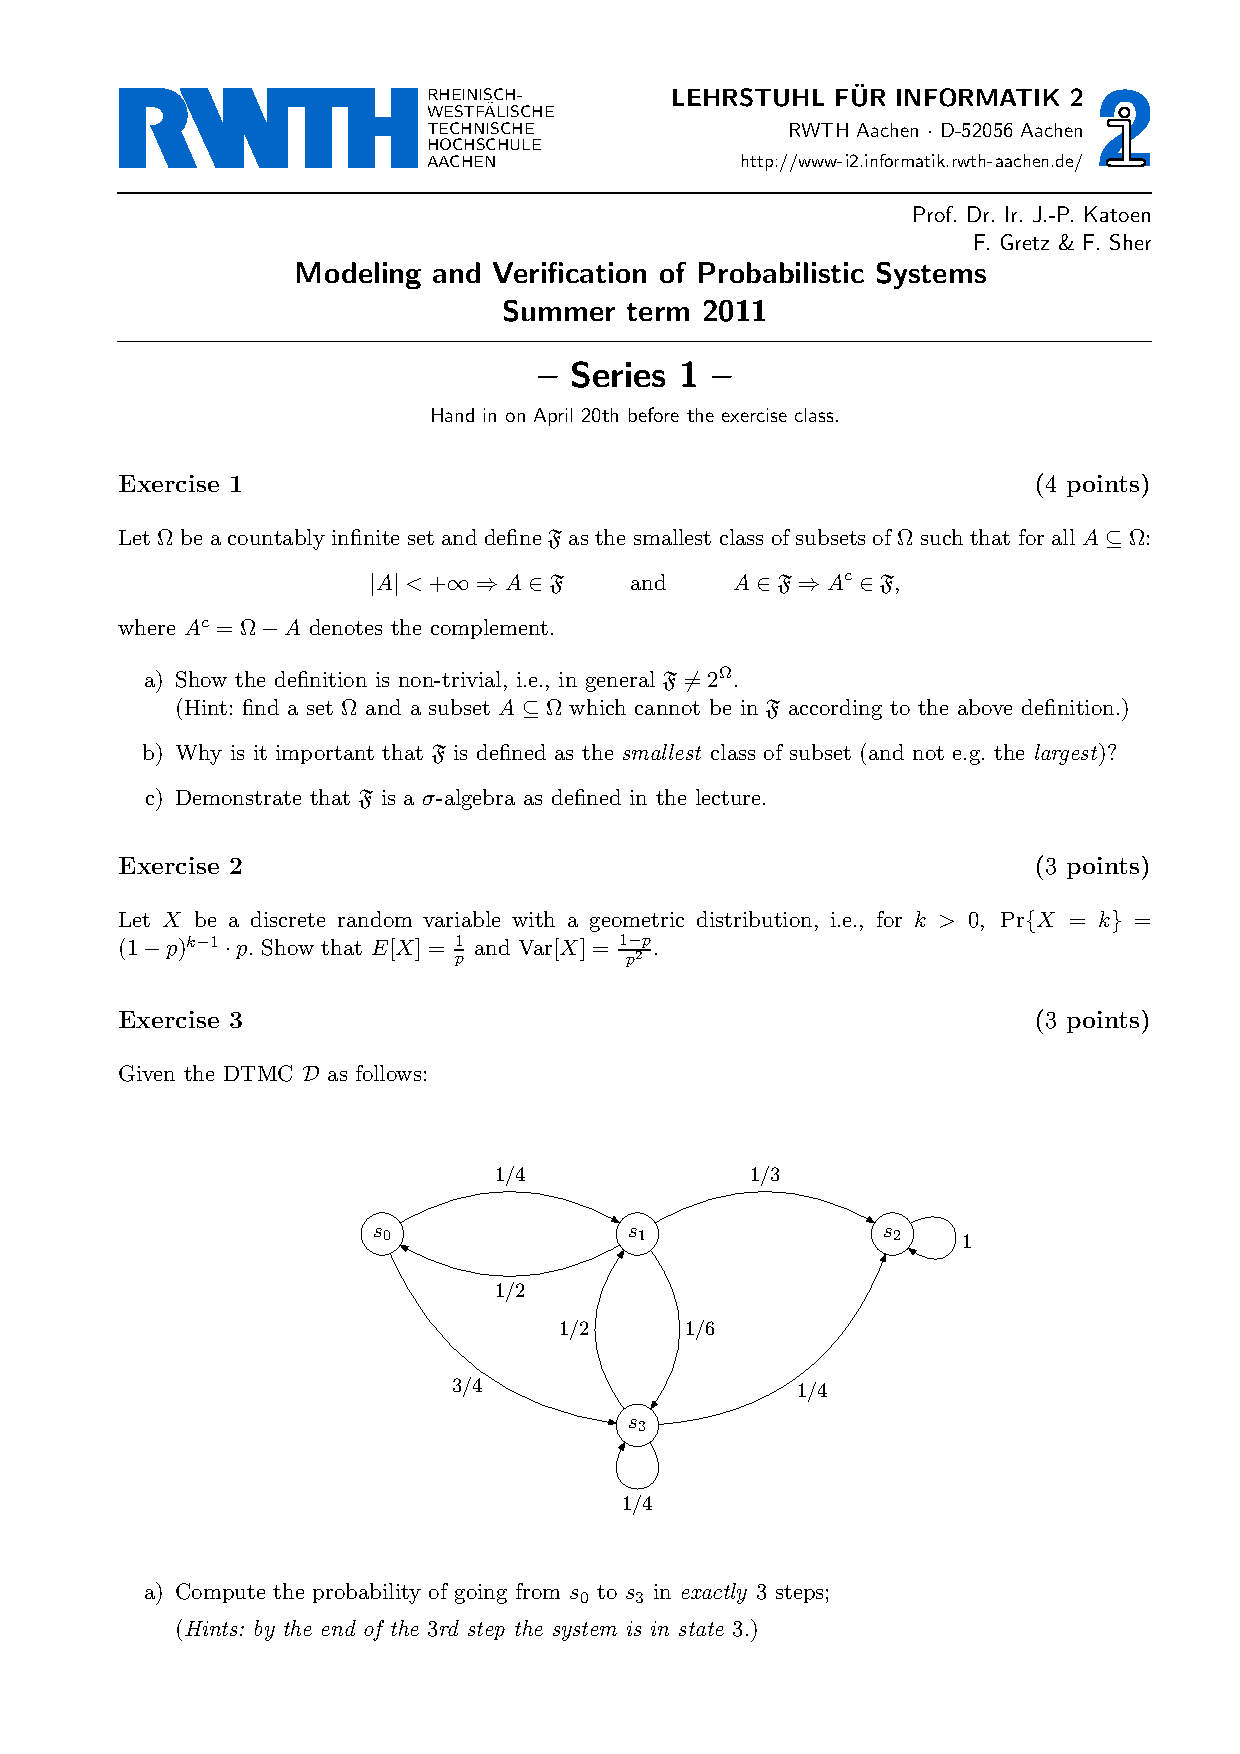
\includepdf[pages={-}]{pdf-to-include/sheet01.pdf}

\subsubsection{Question b}
It is important that $\mathcal{F}$ is defined as the \emph{smallest}
class of subset because the constraint ``smallest'' allow our building
process to stop where we mention before, that is, it allow to not
include pairs of sets $A$ and $A^c$ both infinite. This is the main
difference between $\mathcal{F}$ and $2^\Omega$, having a non trivial
set $\mathcal{F}$.

It is important to note that given $\Omega$ a countably infinite set,
$\mathcal{F}$ is countably infinite too, because the number of finite
sets (which all belong to $\mathcal{F}$) is infinite.

Instead, if the ``largest'' constraint was required, we have to
include as many sets as we can, every pairs of sets $A$ and $A^c$,
both infinite, too. In this way we have $\mathcal{F} = 2^\Omega$, so
the definition of $\mathcal{F}$ would be trivial.

\subsubsection{Question c}
Recall the definition of $\sigma$-algebra: a pair $(\Omega,
\mathcal{F})$, with $\Omega \not = \emptyset$ and $\mathcal{F}
\subseteq 2^\Omega$, is a $\sigma$-algebra if:
\begin{enumerate}
\item $\Omega \in \mathcal{F}$
\item $A \in \mathcal{F} \rightarrow A^c \in \mathcal{F}$
\item $\left( \forall i\in\{1,\ldots, n\}: A_i \in \mathcal{F} \right)
  \rightarrow \left(\bigcup_{i=1}^{n} A_i \right ) \in \mathcal{F}$
\end{enumerate}
In the following we show that $\mathcal{F}$ is a $\sigma$-algebra.
\begin{proof}
  By our argument of \emph{Question a}, $\Omega \in \mathcal{F}$ holds
  and by rule 2 of $\mathcal{F}$'s definition, $A \in \mathcal{F}
  \rightarrow A^c \in \mathcal{F}$ holds too. For the last point we
  reason case by case, given $A_i, A_j$ sets both in $\mathcal{F}$:
  \begin{itemize}
  \item if $A_i$ and $A_j$ are both finite, the union of finite sets
    is also finite, hence by rule 1 of $\mathcal{F}$'s definition,
    $A_i \cup A_j \in \mathcal{F}$ holds;
  \item if $A_i$ is finite and $A_j$ is infinite, their union is
    infinite (that is, $A_i \cup A_j$ is the complement of some finite
    set $A_k$). But given an infinite set $A$, we saw before that $A
    \in \mathcal{F} \leftrightarrow |A^c| < \infty$ holds. Using rule
    1, $|A^c| < \infty \rightarrow A^c \in \mathcal{F}$ and so $A_i
    \cup A_j \in \mathcal{F}$ too;
  \item if $A_i$ and $A_j$ are infinite (they're the complements of
    some finite sets $A_i^c, A_j^c$ respectively), their union is
    infinite, so we apply the argument given in the previous point.
  \end{itemize}
\end{proof}

\subsection{Exercise 3}
\subsubsection{Question a}
We type it directly in R:
\begin{lstlisting}
> P <- rbind(c(0, 1/4, 0, 3/4),
+            c(1/2, 0, 1/3, 1/6),
+            c(0, 0, 1, 0),
+            c(0, 1/2, 1/4, 1/4))
> temp <- c(1, 0, 0, 0) # initial distribution all on the zero state
> temp <- temp %*% P # compute the probability distribution after one step
> temp <- temp %*% P # compute the probability distribution after two steps
> temp <- temp %*% P # compute the probability distribution after three steps
> temp # see the result
       [,1]      [,2]     [,3]      [,4]
[1,] 0.1875 0.1458333 0.453125 0.2135417
\end{lstlisting}
The probability to be in $s_3$ starting from $s_0$ in \emph{exactly}
three step is about $.21$.

\subsubsection{Question c}
We type it directly in R:
\begin{lstlisting}
> P <- rbind(c(0, 1/4, 0, 3/4),
+            c(1/2, 0, 1/3, 1/6),
+            c(0, 0, 1, 0),
+            c(0, 1/2, 1/4, 1/4))
> temp <- c(.25, .25, .25, .25) # initial uniform distribution
> temp <- temp %*% P # compute the probability distribution after one step
> temp <- temp %*% P # compute the probability distribution after two steps
> temp <- temp %*% P # compute the probability distribution after three steps
> temp # see the result
           [,1]      [,2]      [,3]      [,4]
[1,] 0.08854167 0.1223958 0.6397569 0.1493056
\end{lstlisting}
The probability to be in $s_2$ in \emph{exactly} three step, assuming
a starting uniform distribution, is about $.63$.


\end{document} 
